\section{Graph Theory} \label{sec:graph-theory}
Many problems in Machine Learning (ML) don't involve classification or prediction of single data points in isolation, but of set of entities that may present a more, or less, complex relation with each other. 
Most real-world phenomena fit into the latter framework.
Graphs are one of the most powerful tools for the modelling of this class of problems, as their structure naturally captures the wide variety of relations that may exist between entities.
These range from the atomical structure of a molecule to a social network of friends.  
In both these examples graphs help in reasoning, visualising and making inferences and predictions.

\subsection{Graphs} \label{subsec:graphs}
\begin{definition}
	A graph is a tuple 
	\begin{equation}
	\mathcal{G} = (\mathcal{V}, \mathcal{E})
\end{equation}
with $\mathcal{V} = \{ v_1 \ldots v_n \}$ the set of \textit{vertices} and $\mathcal{E} = \mathcal{V} \times \mathcal{V}$ the set of \textit{edges}.
\end{definition}

For our scopes, we will only be considering the case where every element in $\mathcal{E}$ is a pair either of the form $(v_i, v_j)$ or $(v_j, v_i)$ with $i \neq j$.  
That is to say that the class of graphs presently of interest for us are those where there can be at most a single directed edge between any node in $\mathcal{V}$ and no self-loops.
We are also interested in enforcing that there be no \textit{cycles} in the graph, i.e. sequences of nodes of the form $v_i \rightarrow v_j \rightarrow \cdots \rightarrow v_i$.
The resulting graph possessing only directed edges and no cycles is commonly called a \textit{directed acyclic graph}, or DAG for short.  
This data structure is of paramount importance as it's the fundamental graphical representation used for Bayesian Networks.

An example of a DAG, containing five nodes, is shown in Fig. \ref{fig:bn-example-dag}.


\begin{figure}[htbp]
\centerline{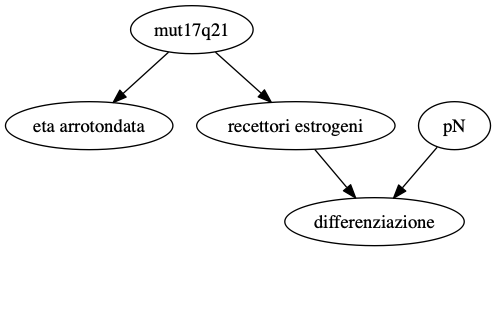
\includegraphics[width=\columnwidth]{mathematical-background/images/bn-example-structure}}
\caption{Example DAG representing a subset of the data set used in this thesis}
\label{fig:bn-example-dag}
\end{figure}

\subsection{Polytrees} \label{subsec:polytrees}
We now have all elements to be able to formally define a Bayesian Network.
I will also define polytrees and trees because these are a fundamental concept for the work carried out in this thesis.
\begin{definition}
	A \textit{loop} is a trace $v_i, v_j \ldots v_i$ of nodes obtained by following edges regardless of their direction
\end{definition}
\begin{definition}
	A directed graph containing no such loops is called a \textit{polytree}. 
\end{definition}
\begin{definition}
	A \textit{tree} is a particular case of polytree where each node has at most one parent.	
\end{definition}

\subsection{D-separation} \label{subsec:d-separation}
\textit{Dependence-separation} or \textit{d-separation}, as the name entails, is a concept relating to the conditional dependence between variables.
It was first presented by \cite{Pearl1988}
To define it, we first have to clarify when two sets of nodes $X$ and $Y$ are causally connected.
This is so if $Z = \emptyset$ and they are part of one of the following three structures, called \textit{v-structures} in this context:
\begin{itemize}
  \item $X \rightarrow Z \rightarrow Y$
  \item $X \leftarrow Z \leftarrow Y$
  \item $X \leftarrow Z \rightarrow Y$
\end{itemize}
This means that knowing something about $X$ also tells us something new about $Y$.
$X$ and $Y$ are causally independent if they appear in the following v-structure:
\begin{itemize}
  \item $X \rightarrow Z \leftarrow  Y$
\end{itemize}
Such a configuration is called a \textit{collider} and it blocks the flow of information from $X$ to $Y$.
If $Z \neq \emptyset$ the cases are reversed so colliders are open and the other three structures are blocked.
\begin{definition}
	Given disjoint subsets $X, Y, Z \subset \mathcal{X}$, $X$ and $Y$ are d-separated if:
	\begin{itemize}
		\item $Z \neq \emptyset$: no path between $X$ and $Y$ presents a collider
		\item $Z = \emptyset$: there is a collider on every path between $X$ and $Y$
	\end{itemize}
\end{definition}

The independencies between variables are encoded in the structure of the DAG so every distribution whose BN has the same connections between nodes also has the same independencies, regardless of the values of the variables.

A series of examples using the DAG presented in Fig. \ref{fig:bn-example-dag} are shown in Fig. \ref{fig:bn-separations-example-1}, \ref{fig:bn-separations-example-2}, \ref{fig:bn-separations-example-3}.
We can see how the network's topology and the nodes chosen to be in the observed set $Z$, define the resulting separations.
In all cases $X= \{ \text{eta arrotondata} \}$ and $Y=V \smallsetminus X \smallsetminus Z$; we are asking for the set of all nodes in the DAG that are d-separated from $X$, given evidence $Z$.
The reason for this can easily be done by enumerating all paths through the v-structures in the network and applying the definitions for causal connections given above.
In the case shown in Fig. \ref{fig:bn-separations-example-1} we see that the node \textbf{eta arrotondata} is separated from nodes \textbf{recettori estrogeni}, \textbf{differenziazione} and \textbf{pN} given the observed evidence \textbf{mut17q21}.
The reason for this is because \textbf{$\text{eta arrotondata} \leftarrow \text{mut17q21} \rightarrow \text{recettori estrogeni}$} is a \textit{fork} and thus the flow of information from the rest of the network is blocked.
The way in which changing the conditioning set $Z$ also changes the independencies, can clearly be seen in Fig. \ref{fig:bn-separations-example-2} and \ref{fig:bn-separations-example-3}.

\begin{figure}[htbp]
\centerline{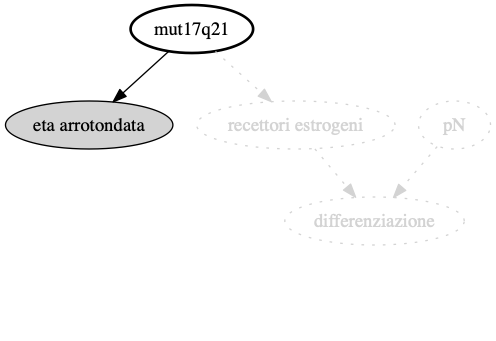
\includegraphics[width=\columnwidth]{mathematical-background/images/bn-example-separations-1}}
\caption{D-Separations in a subset of the provided data set (see Sec. \ref{sec:data-set})}
\label{fig:bn-separations-example-1}
\end{figure}

\begin{figure}[htbp]
\centerline{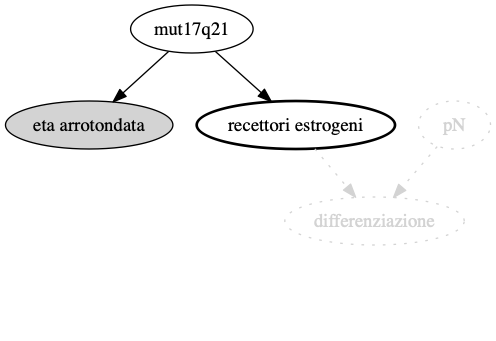
\includegraphics[width=\columnwidth]{mathematical-background/images/bn-example-separations-2}}
\caption{D-Separations in a subset of the provided data set (see Sec. \ref{sec:data-set})}
\label{fig:bn-separations-example-2}
\end{figure}

\begin{figure}[htbp]
\centerline{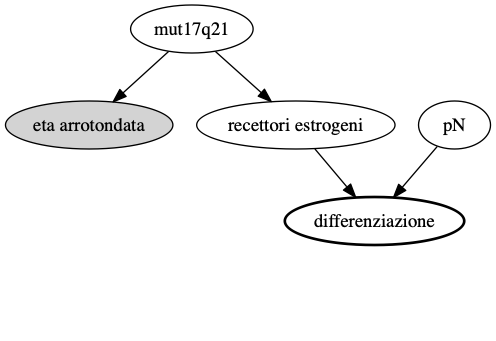
\includegraphics[width=\columnwidth]{mathematical-background/images/bn-example-separations-3}}
\caption{D-Separations in a subset of the provided data set (see Sec. \ref{sec:data-set})}
\label{fig:bn-separations-example-3}
\end{figure}
